\documentclass[../../DD.tex]{subfiles}
\begin{document}
\section{Entity-Relationship Model}

	The Entity Relationship Model (ER Modeling) is a way to graphically design the database. It serves as a high-level data model that defines the data elements and their relationships within a specific system. The ER model is used to represent real-world entities, which are distinguishable objects in their surrounding environment. These entities can have relationships with each other, making the main structure of the database.
    
    Cardinality constraints play an important role during the definition of entities in relationships. They specify the minimum and maximum number of relationships in which an entity can engage. In the diagram, usually the Min-Max notation is used, positioning the cardinality values near the respective entities. It is possible to use the exact number (i.e. the areas in our case cam be defined a priori as 4) or generic number (i.e. if you think that VenTour will increase the number of area field, it can be put simply $N$).
    \begin{figure}[h]
        \centering
        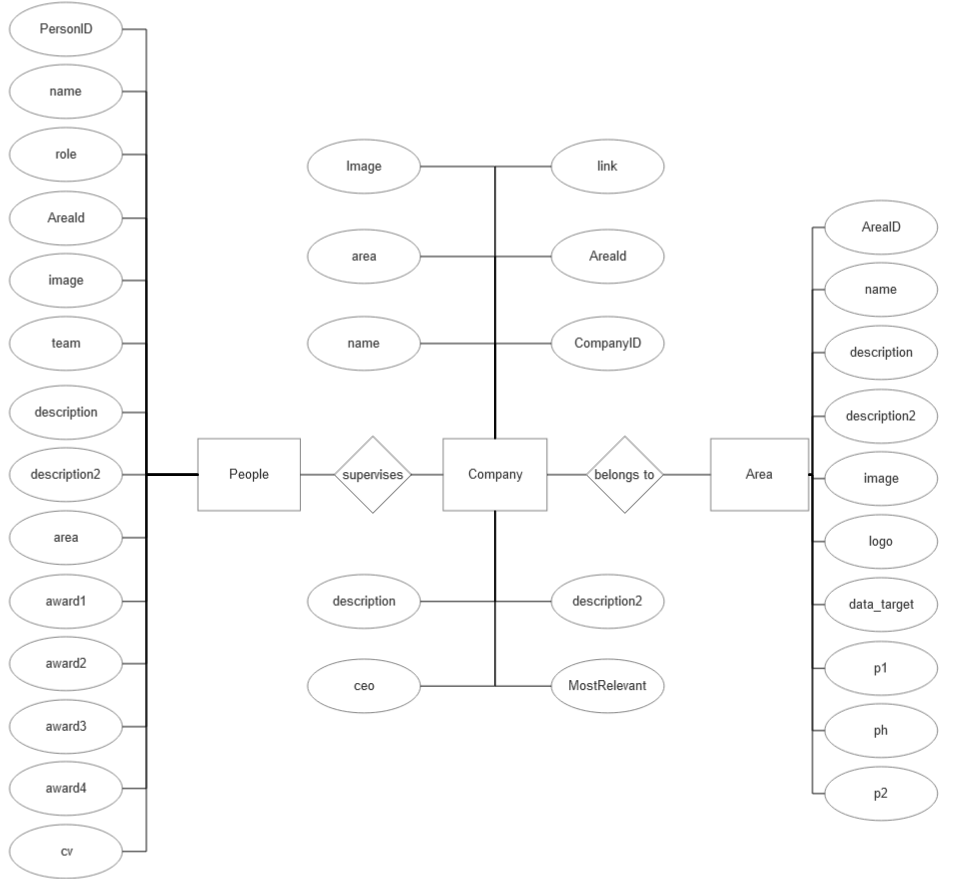
\includegraphics[width=\textwidth]{Images/Database/ERD.png}
        \caption{Entity-Relationship Model}
        \label{fig: ERD}
    \end{figure}
\end{document}
